      %%%%%%%% ICML 2025 EXAMPLE LATEX SUBMISSION FILE %%%%%%%%%%%%%%%%%

\documentclass{article}

% Recommended, but optional, packages for figures and better typesetting:
\usepackage{microtype}
\usepackage{graphicx}
\usepackage{subfigure}
\usepackage{booktabs} % for professional tables

% hyperref makes hyperlinks in the resulting PDF.
% If your build breaks (sometimes temporarily if a hyperlink spans a page)
% please comment out the following usepackage line and replace
% \usepackage{icml2025} with \usepackage[nohyperref]{icml2025} above.
\usepackage{hyperref}


% Attempt to make hyperref and algorithmic work together better:
\newcommand{\theHalgorithm}{\arabic{algorithm}}

% Use the following line for the initial blind version submitted for review:
% \usepackage{icml2025}

% If accepted, instead use the following line for the camera-ready submission:
\usepackage[accepted]{icml2025}

% For theorems and such
\usepackage{amsmath}
\usepackage{amssymb}
\usepackage{mathtools}
\usepackage{amsthm}

% if you use cleveref..
\usepackage[capitalize,noabbrev]{cleveref}

%%%%%%%%%%%%%%%%%%%%%%%%%%%%%%%%
% THEOREMS
%%%%%%%%%%%%%%%%%%%%%%%%%%%%%%%%
\theoremstyle{plain}
\newtheorem{theorem}{Theorem}[section]
\newtheorem{proposition}[theorem]{Proposition}
\newtheorem{lemma}[theorem]{Lemma}
\newtheorem{corollary}[theorem]{Corollary}
\theoremstyle{definition}
\newtheorem{definition}[theorem]{Definition}
\newtheorem{assumption}[theorem]{Assumption}
\theoremstyle{remark}
\newtheorem{remark}[theorem]{Remark}

% Todonotes is useful during development; simply uncomment the next line
%    and comment out the line below the next line to turn off comments
%\usepackage[disable,textsize=tiny]{todonotes}
\usepackage[textsize=tiny]{todonotes}


% The \icmltitle you define below is probably too long as a header.
% Therefore, a short form for the running title is supplied here:
\icmltitlerunning{Analysis Report on "Interpretable Lightweight Transformer via Unrolling of Learned Graph Smoothness Priors"}

\begin{document}

\twocolumn[
\icmltitle{Analysis Report on \textit{Interpretable Lightweight Transformer \\via Unrolling of Learned Graph Smoothness Priors}}

% It is OKAY to include author information, even for blind
% submissions: the style file will automatically remove it for you
% unless you've provided the [accepted] option to the icml2025
% package.

% List of affiliations: The first argument should be a (short)
% identifier you will use later to specify author affiliations
% Academic affiliations should list Department, University, City, Region, Country
% Industry affiliations should list Company, City, Region, Country

% You can specify symbols, otherwise they are numbered in order.
% Ideally, you should not use this facility. Affiliations will be numbered
% in order of appearance and this is the preferred way.
\icmlsetsymbol{equal}{*}

\begin{icmlauthorlist}
\icmlauthor{Kenneth Browder}{ipp}
\icmlauthor{Fabien Lagnieu}{ipp}
\end{icmlauthorlist}

\icmlaffiliation{ipp}{Institut Polytechnique de Paris, France}

\icmlcorrespondingauthor{Kenneth Browder}{kenneth.browder@ip-paris.fr}
\icmlcorrespondingauthor{Fabien Lagnieu}{fabien.lagnieu@polytechnique.edu}

% You may provide any keywords that you
% find helpful for describing your paper; these are used to populate
% the "keywords" metadata in the PDF but will not be shown in the document
\icmlkeywords{Machine Learning, IPP, ML with Graphs, Graph Signal Processing}

\vskip 0.2in
]

% this must go after the closing bracket ] following \twocolumn[ ...

% This command actually creates the footnote in the first column
% listing the affiliations and the copyright notice.
% The command takes one argument, which is text to display at the start of the footnote.
% The \icmlEqualContribution command is standard text for equal contribution.
% Remove it (just {}) if you do not need this facility.

%\printAffiliationsAndNotice{}  % leave blank if no need to mention equal contribution
\printAffiliationsAndNotice{\icmlEqualContribution} % otherwise use the standard text.

\begin{abstract}
This report analyzes the paper \textit{Interpretable Lightweight Transformer via Unrolling of Learned Graph Smoothness Priors} \cite{do2024interpretable}. The authors propose an efficient and interpretable transformer-like model for graph signal interpolation. Their method uses unrolled optimization algorithms based on graph smoothness priors. The first section presents its main contributions, methodology, and experimental results and describe the reproduction of one key experiment and an additional experiment. The second section examines a related paper, discuss its relevance, and compare its approach with the first.
\end{abstract}

\section*{Section 1: Analysis of the Main Paper}

\textit{Interpretable Lightweight Transformer via Unrolling of Learned Graph Smoothness Priors}
\\Tam Thuc Do, Parham Eftekhar, Seyed Alireza Hosseini, Gene Cheung, Philip Chou - Published in June 2024.

\setcounter{section}{1}
\subsection{Introduction}

Transformer architectures are central to modern machine learning, particularly in natural language processing and computer vision. Despite their success, they face two main limitations: high computational cost and lack of interpretability. These issues restrict their use in resource-constrained settings or applications requiring transparency.

The paper proposes a simple and effective solution by combining Graph Signal Processing (GSP) with neural network architectures. GSP models data structured as graphs by leveraging their relational information. The authors unroll optimization algorithms for graph signal interpolation into a neural network, resulting in a transformer-like model that is both lightweight and interpretable.

\subsection{State of the Art}

Graph-based learning has made important progress in recent years, so many methods focus on learning from data structured as graphs. GSP provides a solid framework for analyzing such data, it extends traditional signal processing tools to irregular graph domains and allows processing signals that live on nodes of a graph by using the graph structure \cite{shuman2013emerging}.

Two key tools in GSP are the Graph Laplacian Regularizer (GLR) and Graph Total Variation (GTV). GLR promotes smoothness, encouraging similar values for connected nodes \cite{ortega2018graph}. In contrast, GTV allows sharp changes and preserves edges and discontinuities \cite{cheung2018graph}.

In the analyzed paper, GLR and GTV guide both graph learning and signal interpolation, ensuring smoothness and edge preservation in the reconstructed signals.

\subsection{Main Contributions of the Proposed Method}

The proposed method rethinks the transformer paradigm by integrating graph learning and optimization unrolling into a unified framework for graph signal interpolation. Its core contributions are outlined below.

\subsubsection{Overview of the Transformer-like Architecture}

The architecture alternates between learning a similarity graph and updating the interpolated signal. At each layer, the graph and signal are refined through an unrolled optimization process. This iterative structure mimics transformers but relies on graph-based operations, ensuring interpretability and lower complexity.

\subsubsection{Graph Learning via Mahalanobis Distance}

The graph learning module constructs a similarity graph by computing pairwise distances between nodes. It uses the \textit{Mahalanobis distance} \cite{hu2020feature}, which measures the similarity between two feature vectors $\mathbf{f}_i$ and $\mathbf{f}_j$.

The \textit{Mahalanobis distance} between two nodes $i$ and $j$ is defined as: $d(i, j) = (\mathbf{f}_i - \mathbf{f}_j)^\top \mathbf{M} (\mathbf{f}_i - \mathbf{f}_j)$, where $\mathbf{M}$ is a learnable, positive semi-definite matrix that adapts the metric to the data during training. And the edge weights $w_{i,j}$ between nodes are computed as: $w_{i,j} = \exp(-d(i,j)).$ A local softmax normalizes outgoing edges so their weights sum to one, similar to transformer attention.

This approach guarantees the symmetry of the learned graph and provides an interpretable alternative to the key-query-value attention commonly used in standard transformers.

\subsubsection{Optimization Unrolling for Signal Interpolation}

Once the graph is defined, the model performs signal interpolation guided by graph smoothness priors. Two optimization strategies are employed: the \textit{Conjugate Gradient} (CG) method used to minimize the $\ell_2$-norm GLR \cite{shewchuk1994introduction} and the \textit{Alternating Direction Method of Multipliers} (ADMM) applied to minimize the $\ell_1$-norm GTV \cite{wang2017new}.

\begin{figure}[ht]
\vskip -0.1in
\begin{center}
\centerline{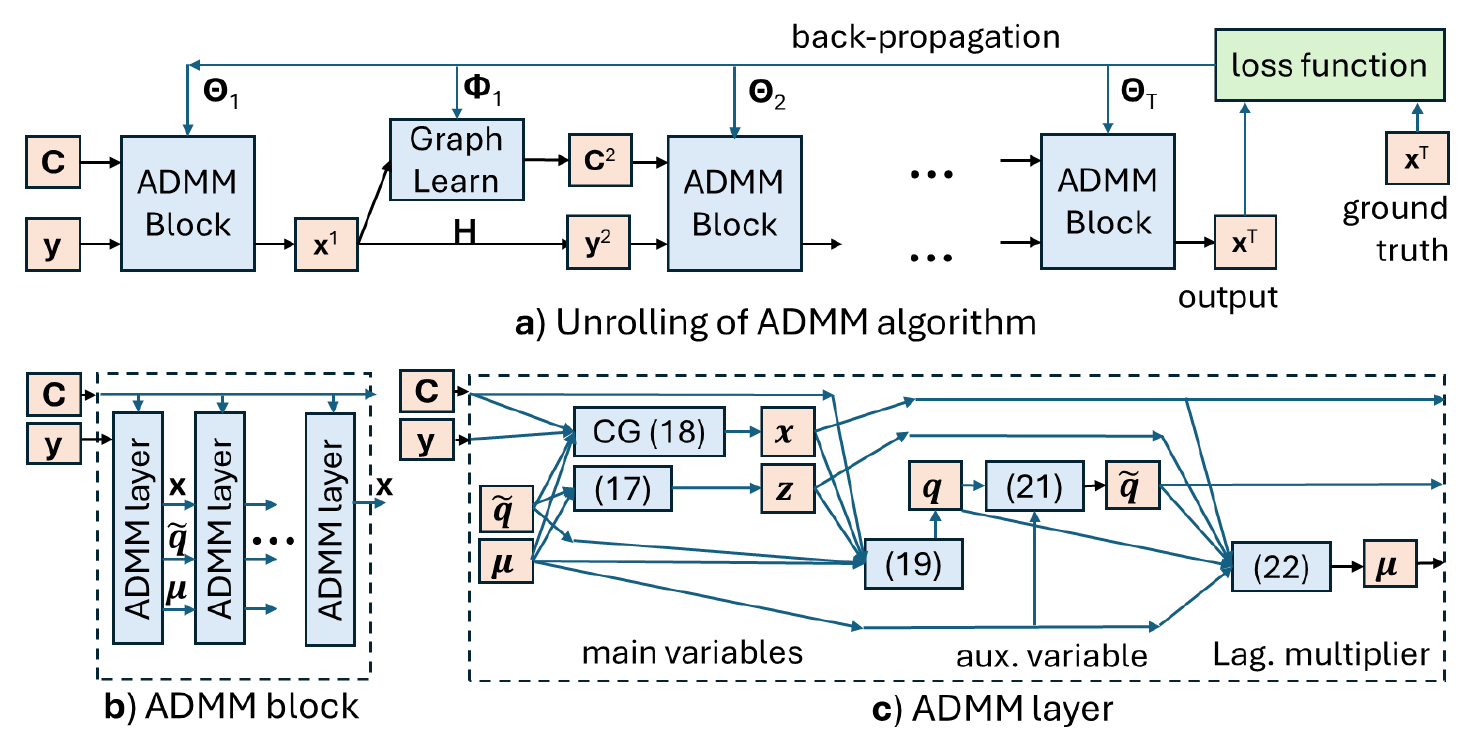
\includegraphics[width=\columnwidth]{GTV-based_algorithm.png}}
\caption{Unrolling of GTV-based signal interpolation algorithm \cite{do2024interpretable}.}
\label{fig:unrolling-gtv}
\end{center}
\vskip -0.3in
\end{figure}

Each iteration of these algorithms is implemented as a neural network layer, enabling end-to-end training through backpropagation.

\subsubsection{Interpretability and Efficiency}

Each layer performs a well-defined, interpretable operation, replacing traditional self-attention with a graph learning module guided by graph smoothness priors, avoiding the opacity of key-query-value mechanisms.

By leveraging unrolled optimization and efficient graph-based operations, the model eliminates large parameter matrices, reducing computational cost while maintaining strong performance.

This model advances the state of the art by showing that transformer-like architectures can achieve competitive performance with fewer parameters, while offering greater interpretability than conventional attention mechanisms.

\subsection{Experimental Validation}

\subsubsection{Experimental Setup}

All experiments are implemented in PyTorch. Models are trained on the DIV2K dataset, containing 800 high-resolution (HR) training images and 100 validation images. To reduce computational cost, the authors extract $64 \times 64$ pixel patches and sample only $1\%$ to $4\%$ of all available patches for training. Testing is performed on three standard benchmarks: McM \cite{zhang2011color}, Kodak \cite{kodak1993}, and Urban100 \cite{huang2015single}.

Two tasks are considered: \textit{Image Interpolation} (reconstructing high-resolution images from sparsely sampled data) and \textit{Demosaicking} (reconstructing full-color images from Bayer-patterned inputs).

Performance is evaluated using Peak Signal-to-Noise Ratio (PSNR) and Structural Similarity Index Measure (SSIM) \cite{wang2004image}.

\subsubsection{Results on Image Interpolation}

The authors evaluate their models on image interpolation tasks. The proposed models, uGLR and uGTV, are compared to established methods including MAIN \cite{ji2020image} and SwinIR-lightweight \cite{liang2021swinir}, as well as a simple Bicubic interpolation baseline.

uGTV consistently achieves the best PSNR and SSIM scores across all datasets. Notably, it outperforms MAIN and SwinIR, despite having significantly fewer parameters (319k versus 10.9M for MAIN and 0.9M for SwinIR).

\subsubsection{Results on Demosaicking}

\begin{table}[b]
\vskip -0.3in
\caption{Demosaicking performance (PSNR / SSIM) for selected models, trained on 10k samples from DIV2K.}
\label{tab:demosaicking_selected}
\begin{center}
\begin{small}
\begin{sc}
\begin{tabular}{lccc}
\toprule
\textbf{Method} & \textbf{Params \#} & \textbf{Kodak} & \textbf{Urban100} \\
\midrule
Bilinear  & -        &  28.22 / 0.890 & 24.18 / 0.873 \\
RST-B & 931,763   &  38.75 / 0.986 & 32.82 / 0.973 \\
RST-S & 3,162,211 &  \textbf{39.81} / \textbf{0.988} & 33.87 / 0.978 \\
uGLR  & 323,410   &  37.88 / 0.982 & 33.60 / 0.977 \\
uGTV  & 323,435   &  39.11 / 0.986 & \textbf{34.01} / \textbf{0.979} \\
\bottomrule
\end{tabular}
\end{sc}
\end{small}
\end{center}
\vskip -0.2in
\end{table}

For demosaicking, uGTV shows competitive performance with a lightweight design. Table~\ref{tab:demosaicking_selected} presents selected results on the Kodak and Urban100 datasets. To maintain readability, only the most relevant models (Bilinear, RSTCANet-B/S \cite{xing2022residual}, uGLR, and uGTV) are reported.

uGTV achieves top PSNR and SSIM on Urban100 and closely matches RST-S on Kodak, while using nearly ten times fewer parameters. These results confirm uGTV’s balance between accuracy and efficiency. Its performance generalizes well across datasets without complex architectures.

\subsubsection{Robustness to Covariate Shift}

The authors also assess the robustness of their models under covariate shift by adding Gaussian noise to the inputs during testing. Table~\ref{tab:robustness} shows the demosaicking PSNR values for different noise levels ($\sigma$). uGTV consistently outperforms RST-B, especially as noise increases.
\begin{table}[t]
\caption{Demosaicking performance (PSNR) under Gaussian noise (trained on noiseless data).}
\label{tab:robustness}
\vskip -0.2in
\begin{center}
\begin{small}
\begin{sc}
\begin{tabular}{lcccc}
\toprule
\textbf{Method} & $\sigma=10$ & $\sigma=20$ & $\sigma=30$ & $\sigma=50$ \\
\midrule
RST-B & 28.01 & 22.70 & 19.34 & 15.03 \\
uGLR & 28.24 & 22.84 & 19.49 & 15.20 \\
uGTV & \textbf{28.31} & \textbf{22.89} & \textbf{19.56} & \textbf{15.38} \\
\bottomrule
\end{tabular}
\end{sc}
\end{small}
\end{center}
\vskip -0.2in
\end{table}

These results confirm that both uGLR and uGTV are more robust to noise compared to RST-B, with uGTV showing the best stability across all tested noise levels.

\subsubsection{Discussion}

The experimental results confirm the effectiveness of the proposed method. Despite having significantly fewer parameters, uGLR and uGTV outperform or match the performance of more complex models like RSTCANet and MAIN. Additionally, they demonstrate better robustness under covariate shifts.

\subsection{Reproduction and Additional Experiments}

In this section, we describe the experiments we performed to reproduce the key results of the paper, and an additional experiment designed to assess the robustness and generalization capabilities of the proposed method.

\subsubsection{Reproduction of a Key Experiment}

%%%%%%%%%%%%%%%%%%%%%%%%%%%%%%%%%%%%%%% Kenneth %%%%%%%%%%%%%%%%%%%%%%%%%%%%%%%%%%%%%%%%%%%%%%%%

\textbf{Objective}: Validate the demosaicking performance of the proposed uGTV model on the ZzZzZ dataset.

\textbf{Methodology}: ZzZzZ ZzZzZ ZzZzZ ZzZzZ ZzZzZ ZzZzZ ZzZzZ 

\textbf{Results}: ZzZzZ ZzZzZ ZzZzZ ZzZzZ ZzZzZ ZzZzZ 

\textbf{Discussion}: ZzZzZ ZzZzZ ZzZzZ ZzZzZ ZzZzZ ZzZzZ 

\subsubsection{Additional Experiment}

\textbf{Objective}: ZzZzZ ZzZzZ ZzZzZ ZzZzZ ZzZzZ 

\textbf{Methodology}: ZzZzZ ZzZzZ ZzZzZ ZzZzZ ZzZzZ 

\textbf{Results}: ZzZzZ ZzZzZ ZzZzZ ZzZzZ ZzZzZ 

\textbf{Discussion}: ZzZzZ ZzZzZ ZzZzZ ZzZzZ ZzZzZ 

Further details on these experiments are provided in the appendix. The full codebase is available at:
\begin{center}
\vskip -0.1in
\href{https://github.com/XwaeK/ML_with_Graphs_Project.git}{\textbf{\texttt{https://github.com/XwaeK/\\ML\_with\_Graphs\_Project.git}}}
\vskip -0.1in
\end{center}

\subsection{Critical Analysis}

The proposed model successfully combines interpretability, computational efficiency, and strong empirical results, achieving state-of-the-art performance with significantly fewer parameters.

However, its scalability to very large graphs remains uncertain, and it has so far only been applied to image-based signal interpolation and demosaicking tasks; future work could explore its extension to more diverse graph learning problems such as node classification or link prediction.


\setcounter{section}{2}
\setcounter{subsection}{0}
\section*{Section 2: Analysis of a Related Paper}

\textit{Inpainting-Driven Graph Learning via Explainable Neural Networks}
\\Minh Trieu Trinh, Tam V. Nguyen, Thanh-Toan Do, Dinh Phung, Svetha Venkatesh - Published in 2024.

%%%%%%%%%%%%%%%%%%%%%%%%%%%%%%%%%%%%%%% Kenneth %%%%%%%%%%%%%%%%%%%%%%%%%%%%%%%%%%%%%%%%%%%%%%%%

\subsection{ZzZzZ ZzZzZ Kenneth ZzZzZ ZzZzZ}






\newpage
\bibliography{biblio}
\bibliographystyle{icml2025}


%%%%%%%%%%%%%%%%%%%%%%%%%%%%%%%%%%%%%%%%%%%%%%%%%%%%%%%%%%%%%%%%%%%%%%%%%%%%%%%
%%%%%%%%%%%%%%%%%%%%%%%%%%%%%%%%%%%%%%%%%%%%%%%%%%%%%%%%%%%%%%%%%%%%%%%%%%%%%%%
% APPENDIX
%%%%%%%%%%%%%%%%%%%%%%%%%%%%%%%%%%%%%%%%%%%%%%%%%%%%%%%%%%%%%%%%%%%%%%%%%%%%%%%
%%%%%%%%%%%%%%%%%%%%%%%%%%%%%%%%%%%%%%%%%%%%%%%%%%%%%%%%%%%%%%%%%%%%%%%%%%%%%%%
\newpage
\appendix
\onecolumn
\section{You \emph{can} have an appendix here.}

You can have as much text here as you want. The main body must be at most $8$ pages long.
For the final version, one more page can be added.
If you want, you can use an appendix like this one.  

The $\mathtt{\backslash onecolumn}$ command above can be kept in place if you prefer a one-column appendix, or can be removed if you prefer a two-column appendix.  Apart from this possible change, the style (font size, spacing, margins, page numbering, etc.) should be kept the same as the main body.
%%%%%%%%%%%%%%%%%%%%%%%%%%%%%%%%%%%%%%%%%%%%%%%%%%%%%%%%%%%%%%%%%%%%%%%%%%%%%%%
%%%%%%%%%%%%%%%%%%%%%%%%%%%%%%%%%%%%%%%%%%%%%%%%%%%%%%%%%%%%%%%%%%%%%%%%%%%%%%%


\end{document}


% This document was modified from the file originally made available by
% Pat Langley and Andrea Danyluk for ICML-2K. This version was created
% by Iain Murray in 2018, and modified by Alexandre Bouchard in
% 2019 and 2021 and by Csaba Szepesvari, Gang Niu and Sivan Sabato in 2022.
% Modified again in 2023 and 2024 by Sivan Sabato and Jonathan Scarlett.
% Previous contributors include Dan Roy, Lise Getoor and Tobias
% Scheffer, which was slightly modified from the 2010 version by
% Thorsten Joachims & Johannes Fuernkranz, slightly modified from the
% 2009 version by Kiri Wagstaff and Sam Roweis's 2008 version, which is
% slightly modified from Prasad Tadepalli's 2007 version which is a
% lightly changed version of the previous year's version by Andrew
% Moore, which was in turn edited from those of Kristian Kersting and
% Codrina Lauth. Alex Smola contributed to the algorithmic style files.
